\documentclass{sigchi}

% Use this command to override the default ACM copyright statement
% (e.g. for preprints).  Consult the conference website for the
% camera-ready copyright statement.


%% EXAMPLE BEGIN -- HOW TO OVERRIDE THE DEFAULT COPYRIGHT STRIP -- (July 22, 2013 - Paul Baumann)
% \toappear{Permission to make digital or hard copies of all or part of this work for personal or classroom use is      granted without fee provided that copies are not made or distributed for profit or commercial advantage and that copies bear this notice and the full citation on the first page. Copyrights for components of this work owned by others than ACM must be honored. Abstracting with credit is permitted. To copy otherwise, or republish, to post on servers or to redistribute to lists, requires prior specific permission and/or a fee. Request permissions from permissions@acm.org. \\
% {\emph{CHI'14}}, April 26--May 1, 2014, Toronto, Canada. \\
% Copyright \copyright~2014 ACM ISBN/14/04...\$15.00. \\
% DOI string from ACM form confirmation}
%% EXAMPLE END -- HOW TO OVERRIDE THE DEFAULT COPYRIGHT STRIP -- (July 22, 2013 - Paul Baumann)


% Arabic page numbers for submission.  Remove this line to eliminate
% page numbers for the camera ready copy 

%\pagenumbering{arabic}

% Load basic packages
\usepackage{balance}  % to better equalize the last page
\usepackage{graphics} % for EPS, load graphicx instead 
%\usepackage[T1]{fontenc}
\usepackage{txfonts}
\usepackage{times}    % comment if you want LaTeX's default font
\usepackage[pdftex]{hyperref}
% \usepackage{url}      % llt: nicely formatted URLs
\usepackage{color}
\usepackage{textcomp}
\usepackage{booktabs}
\usepackage{ccicons}
\usepackage{todonotes}

% custom packages
\usepackage{paralist}

% llt: Define a global style for URLs, rather that the default one
\makeatletter
\def\url@leostyle{%
  \@ifundefined{selectfont}{\def\UrlFont{\sf}}{\def\UrlFont{\small\bf\ttfamily}}}
\makeatother
\urlstyle{leo}

% To make various LaTeX processors do the right thing with page size.
\def\pprw{8.5in}
\def\pprh{11in}
\special{papersize=\pprw,\pprh}
\setlength{\paperwidth}{\pprw}
\setlength{\paperheight}{\pprh}
\setlength{\pdfpagewidth}{\pprw}
\setlength{\pdfpageheight}{\pprh}

% Make sure hyperref comes last of your loaded packages, to give it a
% fighting chance of not being over-written, since its job is to
% redefine many LaTeX commands.
\definecolor{linkColor}{RGB}{6,125,233}
\hypersetup{%
  pdftitle={SIGCHI Conference Proceedings Format},
  pdfauthor={LaTeX},
  pdfkeywords={SIGCHI, proceedings, archival format},
  bookmarksnumbered,
  pdfstartview={FitH},
  colorlinks,
  citecolor=black,
  filecolor=black,
  linkcolor=black,
  urlcolor=linkColor,
  breaklinks=true,
}

% create a shortcut to typeset table headings
% \newcommand\tabhead[1]{\small\textbf{#1}}

% End of preamble. Here it comes the document.
\begin{document}

\title{Effects of In-Video Quizzes on MOOC Lecture Viewing}

\numberofauthors{3}
\author{%
  \alignauthor{1st Author Name\\
    \affaddr{Affiliation}\\
    \affaddr{City, Country}\\
    \email{e-mail address}}\\
  \alignauthor{2nd Author Name\\
    \affaddr{Affiliation}\\
    \affaddr{City, Country}\\
    \email{e-mail address}}\\
  \alignauthor{3rd Author Name\\
    \affaddr{Affiliation}\\
    \affaddr{City, Country}\\
    \email{e-mail address}}\\
}

\maketitle

\begin{abstract}

Online courses on sites such as Coursera use quizzes embedded inside lecture videos (\textit{in-video quizzes}) to help learners test their understanding of the video. This paper analyzes how users interact with in-video quizzes, and how in-video quizzes influence users' lecture viewing behavior. We analyze the viewing logs of users who took the Machine Learning course on Coursera. We find that in-video quizzes are a common source and destination of video seeks. These seeks may reflect behaviors such as searching for answers to quizzes within the video. We observe spikes in view counts in portions of the video surrounding in-video quizzes, as a result of reviewing and rewatching. Some users appear to use quiz-oriented video navigation strategies, such as seeking directly from the start of the video to in-video quizzes, or skipping from one in-video quiz to the next. We discuss implications that our findings have on the design of online courses and lecture-viewing platforms. % and MOOC platforms. % Other sources of seeks to in-video quizzes include the preceding section, where the learner may have found an answer. Potential design implications for video-viewing interfaces include making sure that users are easily able to refer to in-video quizzes. % suggest that video-viewing interface designs should make it easy for learners to refer to in-video quizzes. % Our findings that learners' rewatching and seeking activity peaks near in-video quizzes suggests that interfaces should enable learners to easily refer back to in-video quizzes.

%Online courses on sites such as Coursera use quizzes embedded inside lecture videos (\textit{in-video quizzes}) to test learners' understanding of the video. This paper analyzes how users interact with in-video quizzes, and how in-video quizzes influence users' lecture viewing behavior. We analyze the viewing logs of users who took the Machine Learning course on Coursera. We find that video seeks frequently originate from or terminate near in-video quizzes. These seeks are symptomatic of behaviors such as searching for answers to quizzes within the video. We observe spikes in view counts in portions of the video surrounding in-video quizzes, as a result of reviewing and rewatching. Some users appear to use quiz-oriented video navigation strategies, such as jumping directly from the start of the video to the in-video quizzes, or from one in-video quiz to the next. We discuss implications that our findings have on the design of online courses and MOOC platforms. % Other sources of seeks to in-video quizzes include the preceding section, where the learner may have found an answer. Potential design implications for video-viewing interfaces include making sure that users are easily able to refer to in-video quizzes. % suggest that video-viewing interface designs should make it easy for learners to refer to in-video quizzes. % Our findings that learners' rewatching and seeking activity peaks near in-video quizzes suggests that interfaces should enable learners to easily refer back to in-video quizzes.

\end{abstract}

\keywords{in-video quizzes; lecture viewing; lecture navigation; seeking behaviors; MOOCs}

\category{H.5.m.}{Information Interfaces and Presentation
  (e.g. HCI)}{Miscellaneous}

\section{Introduction}

In-video quizzes, which are commonly found in MOOCs (Massive Open Online Courses) on platforms such as Coursera, are questions that users are asked to answer upon reaching a certain point in the video, as shown in \autoref{fig:coursera}. In-video quizzes are auto-graded -- the majority we observe in courses like Coursera's Machine Learning course are either multiple-choice or multiple-checkbox, though there also exist a few numeric free-response quizzes.

In-video quizzes differ from standard quizzes in that the quizzes are displayed directly in the video viewing interface, so users can easily seek elsewhere upon encountering the quiz -- seeking backward to find answers to the quiz, seeking forward to skip the quiz, etc.
The presence of in-video quizzes inside videos can thus influence users' video viewing behaviors, potentially causing seeking and other nonlinear video navigation behaviors. %non-linear viewing behaviors.

\begin{figure}
%\centering
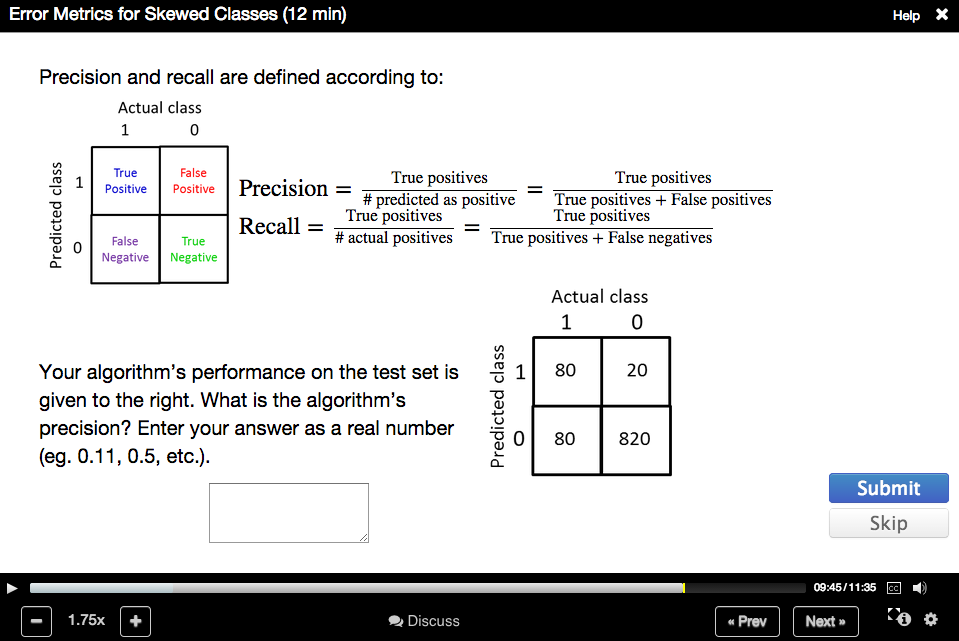
\includegraphics[width=1.0\columnwidth]{coursera}
\caption{An in-video quiz, from the ML4 course on Coursera. In-video quizzes are auto-graded questions embedded into a video and shown at a certain timestamp. They can be either multiple choice, multiple selection, or numeric free-response. Their locations are indicated on the progressbar by a yellow tick.}
\label{fig:coursera}
\end{figure}

In this paper, we analyze video-viewing logs of the fourth iteration of the Machine Learning course on Coursera (ML4). We identify and discuss a set of video viewing behaviors associated with in-video quizzes that we observe in these logs, specifically:

\begin{itemize}
\item The region preceding each in-video quiz is a common destination of video seeks.
\item In-video quizzes are common sources of video seeks.
\item Users often seek backward from in-video quizzes to find the answer to the in-video quiz.
\item Some users appear to be following a strategy of seeking directly to the in-video quizzes
\item Some users tend to jump from one in-video quiz to the next, skipping the video segments
\item Users do not tend to skip over in-video quizzes
\end{itemize}

These behaviors suggest that viewers consider in-video quizzes to be a priority and frequently refer to them. They also suggest that video-viewing interfaces should perhaps make it easier for users to navigate between in-video quizzes and the preceding segment where the answers can be found.

\newpage

\section{Related Work}

Kim et al performed an analysis of reasons for peaks in viewing and seeking while viewing lectures \cite{juho}. They found that users steadily leave videos over time, a phenomenon they refer to as \emph{in-video dropout}, and that visual transitions (such as slide transitions) tend to result in \emph{interaction peaks}, with peaks in events such as users seeking back to the previous slide. They also presented a video viewer that encourages video navigation to interaction peaks  \cite{juho2}. However, the courses that they perform their video log analysis on do not have in-video quizzes, hence they are unable to report on interaction peaks that result from in-video quizzes. We similarly found in our own analysis that there are many peaks in seeking behavior that can be accounted for by slide transitions, however in-video quizzes tend to also be a major factor in causing peaks in video seeking.

Guo and Kim analyzed the effects of video properties such as video length on viewer engagement \cite{guovideo}. They found that users become less engaged as videos grow longer, which is related to the problem of in-video dropout. However, they did not analyze the effects of in-video quizzes on viewer engagement, because the courses they analyzed do not have in-video quizzes. Our findings in this paper suggest that in-video quizzes encourage viewer engagement, as indicated by the increase in rewatching and seeking behavior in the regions of the video surrounding the in-video quiz.

Guo and Reinicke investigated factors that contribute to nonlinear navigation through MOOCs \cite{guodemographics}. They discuss examples of nonlinear navigation such as jumping back to previous lectures, rewatching videos, and going back from assessments to refer to lectures. Our present work is focused on navigation within videos as opposed to within MOOCs. However, we find that in-video quizzes, being a form of assessment that is embedded into the videos, trigger similar backjumps and reviews within a video that Guo and Reinicke discuss at the course-level in their paper.

Anderson et al found that learners differ in the ways they engage with online courses: some only watch videos (``viewers''), some only complete assignments (``solvers''), and some engage in both (``all-rounders'') \cite{ashton}. These differences between learners' engagement patterns are relevant to our work analyzing in-video quizzes, as they help explain why we find that some users' viewing behaviors seem to be aimed towards solving in-video quizzes rather than watching videos.

%  The courses they analyzed were previous offerings of the Machine Learning course on Coursera that is the focus of this work. 
% , and we have found that their findings still apply in the fourth iteration of the course

In-video quizzes are not new; there are many past systems that embed quizzes into multimedia \cite{multimedia}, and they are believed to have positive effects on learning \cite{embedded}. However, to our knowledge, our paper is the first analysis of the effects of in-video quizzes on learners' rewatching and seeking behavior in the context of MOOCs.

\begin{figure}
%\centering
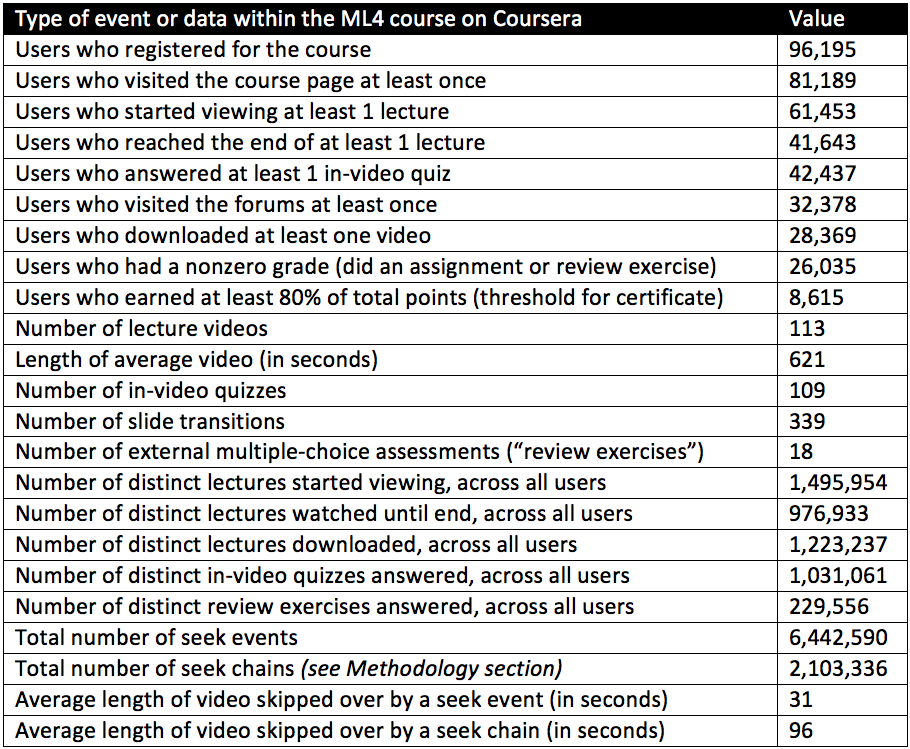
\includegraphics[width=1.0\columnwidth]{summary-statistics}
\caption{Summary statistics for the ML4 course.}
\label{fig:summary-statistics}
\end{figure}

\section{Dataset and Engagement Levels}

The course we are analyzing in this work is the fourth iteration of the Machine Learning course on Coursera (ML4), which ran from October 2013 to January 2014. Our data dump was taken immediately after the course ended. It represents data from 96,195 users, of whom 59,641 watched at least one video. There are 113 lecture videos in the course, totalling 19.5 hours of video content, with an average length of 10 minutes per video.  With 109  in-video quizzes over 19.5 hours of video, this averages out to one in-video quiz for every 11 minutes of video.

Of the 113 videos, 92 videos (81\%) have 1 in-video quiz, 14 videos (12\%) have no in-video quizzes, 6 videos (5\%) have 2 in-video quizzes, and 1 video (1\%) has 3 in-video quizzes. Videos with no in-video quizzes tend to be optional lectures covering interesting applications of machine learning, or are introductory videos that explain what will be covered next in the course. % In videos with 1 in-video quiz, the in-video quiz tends to be placed at the end of the video and is followed by only a summary and no new content. In videos with multiple in-video quizzes, they tend to be evenly spaced out through the video. % Although 60 thousand users began watching the first lecture, the number of viewers drops down to 13 thousand by the midpoint of the course, agreeing with the gradual dropout from courses that previous studies have observed \cite{dropout}.

\begin{figure}
%\centering
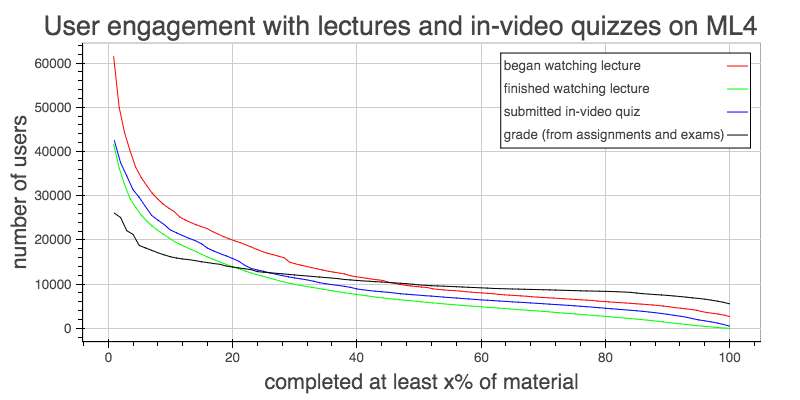
\includegraphics[width=1.0\columnwidth]{user-engagement-with-material}
\caption{Response rates to the 109 in-video quizzes was similar to the viewing rates of the 113 lecture videos.}
\label{fig:user-engagement-with-material}
\end{figure}

Engagement with in-video quizzes was quite high: as shown in \autoref{fig:user-engagement-with-material}, the answering rate of in-video quizzes closely mirrors the watching-completion rate for videos. This contrasts with the lower engagement rates that have typically been found for traditional assignments that are outside of the video \cite{renedisengagement} \cite{ashton}. Other summary statistics are shown in \autoref{fig:summary-statistics}.

% We use viewing logs observed on lectures from ML4 to illustrate certain phenomenon we found to hold true across a wide sample of videos in ML4. One of the lectures we use in our examples is Lecture 68: Error Metrics for Skewed Classes, a 12-minute video containing a single in-video quiz which asks for a free-response numeric answer. Another is Lecture 13: Matrices and vectors, a 9-minute video containing two in-video quizzes, of which the first is multiple-selection (4 checkboxes), and the second is multiple-choice (4 radioboxes).

\section{Methodology}

\subsection{Determining Portions of Video Seen}

The Coursera logs we used for our analysis come with an action (such as play, pause, or seek) associated with a point in the video, and a timestamp. We use these logs to reconstruct the portions of the video that the user has seen, with a technique similar to the one described in \cite{juho} -- if we observe a play event associated with video position p, followed by another event at video position p+i, we can assume that the user watched that segment of the video.

\subsection{Reconstructing Seek Source Positions}

The seek events in Coursera's logs specify only the destination of the seek and the timestamp at which it occurred, but not the origin (the logs tell us where in the video the user seeked to, but not where the user seeked from). However, we were able to reconstruct the seek source positions based on the previous event -- for example, if the user started playing from video position p at timestamp t, and we observe a seek event at timestamp t+i, then we assume the seek originated from video position p+i (or p+2i if the user is playing back the video at 2x speed, etc).

\subsection{Grouping Seek Events into Seek Chains}

Additionally, we observed that many seek events tend to occur in rapid succession as the user narrows down on the actual target. For example, when users seek via the keyboard, if they are at the beginning of the video and their seek target is 3 minutes into the video, they will press the right-arrow repeatedly until they reach the destination, resulting in a large number of small, noisy seek events, rather than the user's intended seek from 0 to 3 minutes that we are interested in analyzing. Because we are primarily interested in where the user ends up seeking to, rather than the individual seek operations that got them to that point, if there are seek events that occur within 5 seconds of one each, we group them together into a single unit which we will call a \textit{seek chain}. Using this approach, we reduced the 6,442,590 total seek events in our dataset into 2,103,336 seek chains. When we analyze seeking in this paper, as well as seek sources and destinations, we will be analyzing seek chains rather than raw seek events, to reduce noise from repeated seeks. That said, our main findings about peaks in seeking around in-video quizzes also hold if we analyze raw seek events instead of seek chains.

% Some play and pause events are automatically generated when the user reaches certain points in the video. For example, when a user clicks on a video in the lecture list, it will auto-play, and a play event is automatically logged at video time 0. When the user reaches an in-video quiz or the end of the video, a pause event is automatically logged at that point. When the user clicks ``continue'' after answering an in-video quiz, the video automatically continues playing, and a play event is logged.

\subsection{Limitations of Coursera's Dataset}

A limitation of Coursera's dataset is that if the user closes their browser window or their network disconnects, this event does not show up in the log, and hence there is ambiguity as to what the user watched. For example, if a user starts playing a video at time t, and this play event is the last logged event, we know that the user must have closed their browser prior to the next in-video quiz or the end of the video (otherwise a pause event would have been logged), however we do not know exactly when the browser was closed. We address this ambiguity by treating it as though the user had immediately stopped watching after that last play event, so we do not include the last (unknown) segment that was watched after their final interaction with the video. %users who quit before the end have watched in the video.

% We observed inconsistencies in the view logs for some users (roughly 1\%) -- for example, observing seek and pause events from the user before we observe any play events -- so we excluded those users from our analysis.

%\section{Engagement levels with }

%\section{In-Video Quiz Answering Rates}

%TODO In this section we analyze:

%\begin{enumerate}
%\item What percent of users who start watching the video reach the in-video quiz? (ie, play a point in the video that is at or past the in-video quiz)
%\item What percent of users who reach the in-video quiz attempt it? What percent skip over it (play a point in the video that is past the in-video quiz, but is not at the quiz)? What percent press the play/skip button (reach the in-video quiz, but continue playing without having submitted an answer)?
%\item What percent of users who attempt in-video quizzes eventually answer them correctly? What is the mean number of tries before a correct answer? What percent of users navigate away from the in-video quiz before answering it correctly? How many navigations away on average?
%\end{enumerate}

%\section{Analysis of Seek Chains via Seek Source and Destination Data}
\section{Aggregate Seek Chain Statistics}

\subsection{Sources and Destinations of Seek Chains}

The sources and destinations of seek chains are shown in \autoref{fig:seek-sources-and-destinations-table}. We see that in-video quizzes are a popular destination of seeks, particularly in the forward direction -- users seek forward to the in-video quiz at 4x the baseline rate of all seek chain destinations. Given the high answering rate for in-video quizzes we showed in \autoref{fig:user-engagement-with-material}, this suggests that these seeks originate from users who want to answer the in-video quiz immediately. Note that Coursera's interface does not have any UI features for seeking to in-video quizzes apart from the progressbar, so the only way to reach the in-video quiz is to seek to a segment of video right before it. Hence, we consider seek chains which terminate at most 10 seconds before the in-video quiz to also represent users intending to do the in-video quiz.

Users also seek backward from in-video quizzes at 55x the baseline rate. As we will show, these represent users reviewing the preceding section, likely trying to find answers to the in-video quiz.

\begin{figure}
%\centering
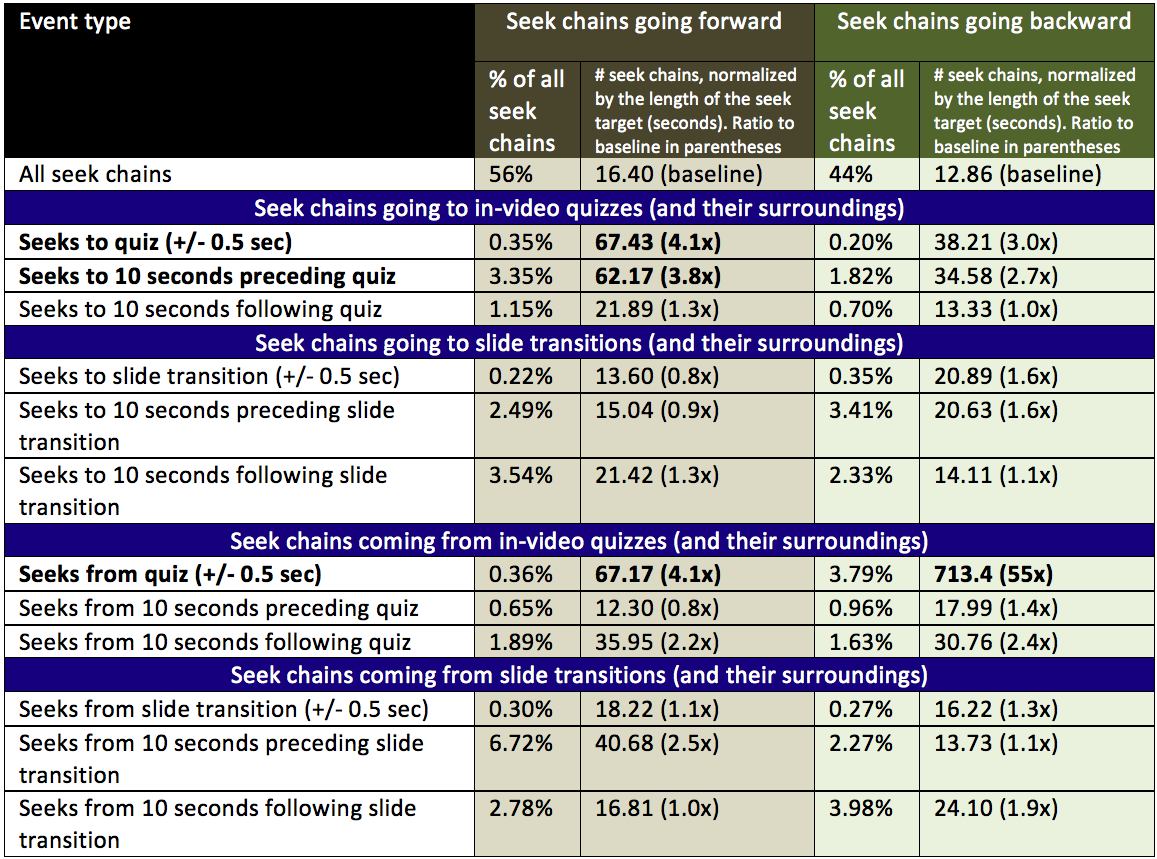
\includegraphics[width=1.0\columnwidth]{seek-sources-and-destinations-table}
\caption{Sources and destinations of seek chains. Users tend to seek backward from in-video quizzes (55x higher than baseline back-seek rate), and forward to in-video quizzes and the 10 seconds immediately preceding them (4x higher than baseline forward-seek rate)}
\label{fig:seek-sources-and-destinations-table}
\end{figure}

%First, we will analyze where users tend to seek to in videos, and what causes them to seek there. Prior work has found that . However, we find that in-video quizzes.

%\subsection{Users Often Seek to In-Video Quizzes}

%If we look at forward seeks in . 

\begin{figure}
%\centering
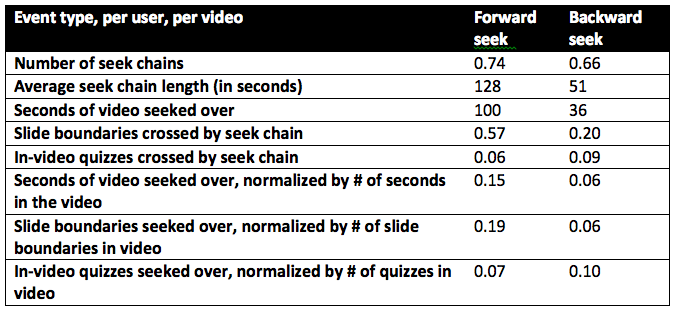
\includegraphics[width=1.0\columnwidth]{table-of-seeks}
\caption{Length of seek chains, and portions of the video that they skip over. Users do not tend to seek forward across in-video quizzes.}
\label{fig:table-of-seeks}
\end{figure}

%\pagebreak

\subsection{Lengths and Directions of Seek Chains}

As shown in \autoref{fig:table-of-seeks}, on average forward seek chains tend to be over longer distances, while backward seek chains tend to be of shorter duration. A potential explanation is that forward seeks aim to go to some salient part of the video -- for example, an in-video quiz -- whereas backward seeks aim to review a part of the video that was just missed. We also observe that users seek forward more than backward overall, including across slide boundaries; however, they tend not to seek forward over in-video quizzes. As we will see, this is because they are seeking to right before the in-video quizzes, either to view the quizzes, or to search for answers to quizzes. %either so that they can do them, or to find information relevant to answering the in-video quiz.

\subsection{Seek Sources and Destinations near In-Video Quizzes}

As we saw in \autoref{fig:seek-sources-and-destinations-table}, there are many seeks with sources and destinations near in-video quizzes. We will look at these seek chains near in-video quizzes in more depth in this section.

\subsubsection{Seek Sources near In-Video Quizzes}

\begin{figure}
%\centering
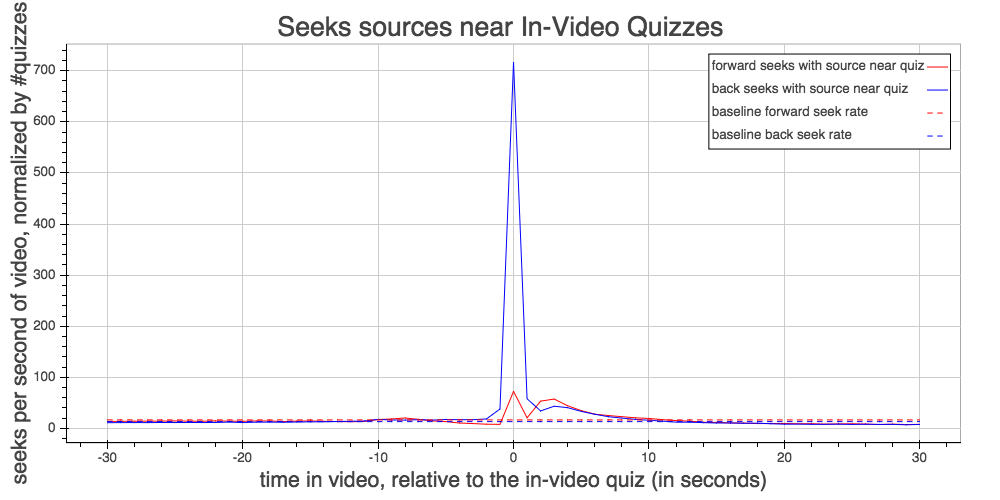
\includegraphics[width=1.0\columnwidth]{seek-sources-near-quizzes}
\caption{Seek chains with sources near in-video quizzes, averaged across all 109 in-video quizzes in the ML class. There are many backward seeks originating at the in-video quiz, reflecting users wanting to review the preceding material.}
\label{fig:seek-sources-near-quizzes}
\end{figure}

\autoref{fig:seek-sources-near-quizzes} illustrates the sources of seek chains near in-video quizzes, averaged across all 109 quizzes. As we can see, there are a large number of backward seeks originating from in-video quizzes. These reflect users who, having seen the in-video quiz, are reviewing the preceding section to find information to help them answer it. However, there are also many forward seeks originating from the in-video quiz as well as the portion that immediately follows it. These likely reflect users who, having looked at or completed the in-video quiz, are seeking forward to preview the next section.

\subsubsection{Seek Destinations near In-Video Quizzes}

\begin{figure}
%\centering
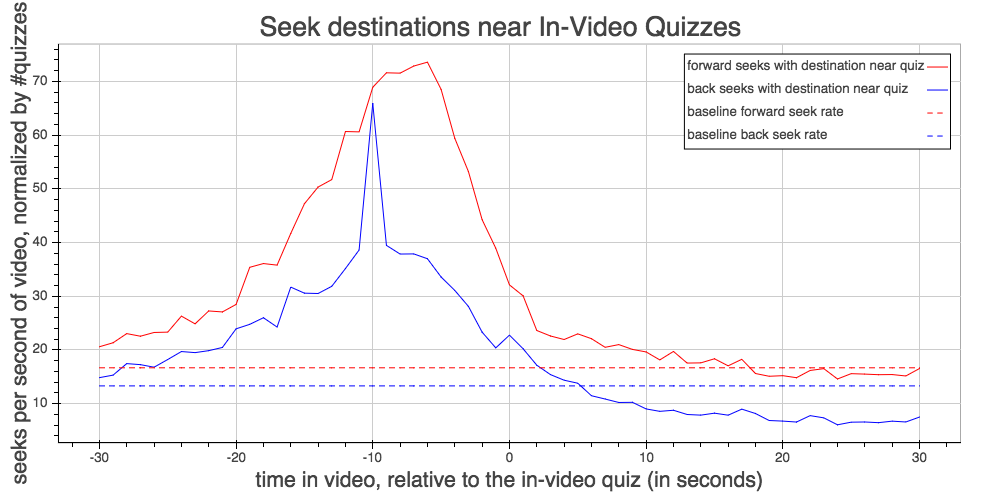
\includegraphics[width=1.0\columnwidth]{seek-destinations-near-quizzes}
\caption{Seek chains with destinations near in-video quizzes, averaged across all 109 in-video quizzes in the ML class. The portion immediately preceding the in-video quiz is a common destination of both forward and backward seeks, perhaps reflecting users who are seeking forward to preview the in-video quiz, or seeking back to find answers to the quiz.}
\label{fig:seek-destinations-near-quizzes}
\end{figure}

\autoref{fig:seek-destinations-near-quizzes} illustrates where users seek to near in-video quizzes, averaged across all 109 quizzes. As we can see, the 10 seconds immediately preceding the in-video quiz are a popular destination of seeks, both in the forward and backward directions. Seek chains in the forward direction arriving just before the in-video quizzes may reflect users who intend to go to the in-video quiz -- Coursera's interface does not provide a means of going to an in-video quiz, other than seeking to the immediately preceding portion and playing the video. Seek chains in the back direction arriving just before the in-video quizzes may reflect users who are reviewing the video to find answers to the in-video quiz. We observe a spike in back-seek destinations at exactly 10 seconds before the in-video quiz. This is likely users who are seeking backwards from the in-video quiz using the back arrow key on their keyboards, which causes a backward seek of exactly 10 seconds.

\section{Viewing Behavior in Individual Lectures}

\subsection{Visualization of Seeks and Watching}

\begin{figure*}
%\centering
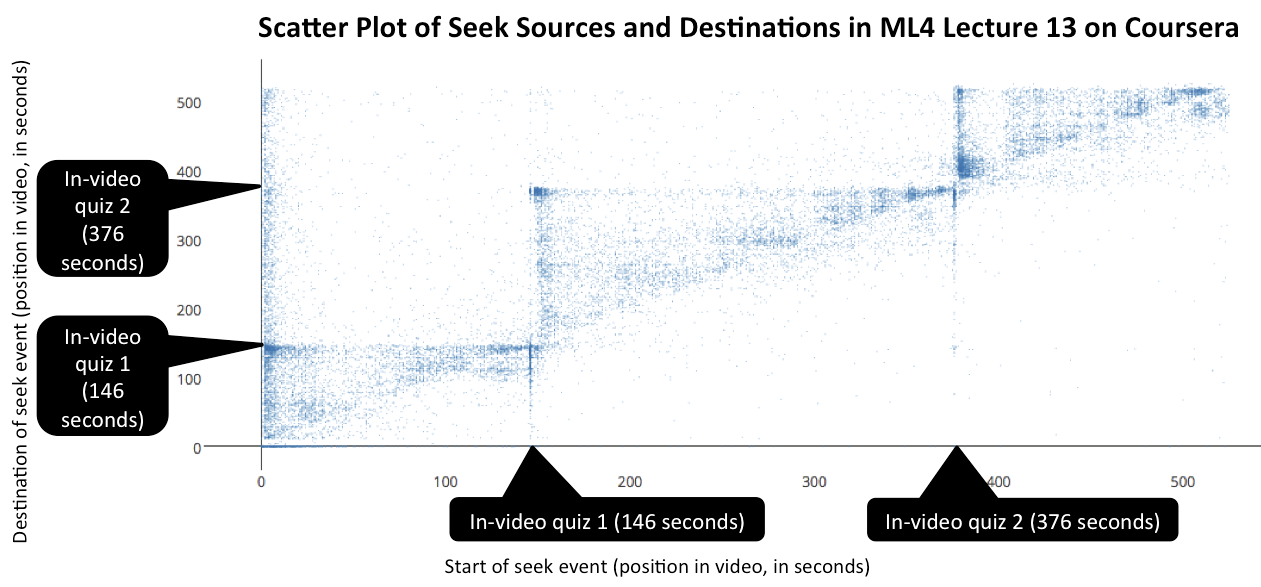
\includegraphics[width=2.0\columnwidth]{scatter-plot-of-seeks}
\caption{Seek sources and destinations in a lecture with 2 in-video quizzes. Each point at (x,y) represents a seek from time x to y. There are many seeks to in-video quizzes from the start of the video, the previous section, and between quizzes.}
\label{fig:scatter-plot-of-seeks}
\end{figure*}

\begin{figure*}
%\centering
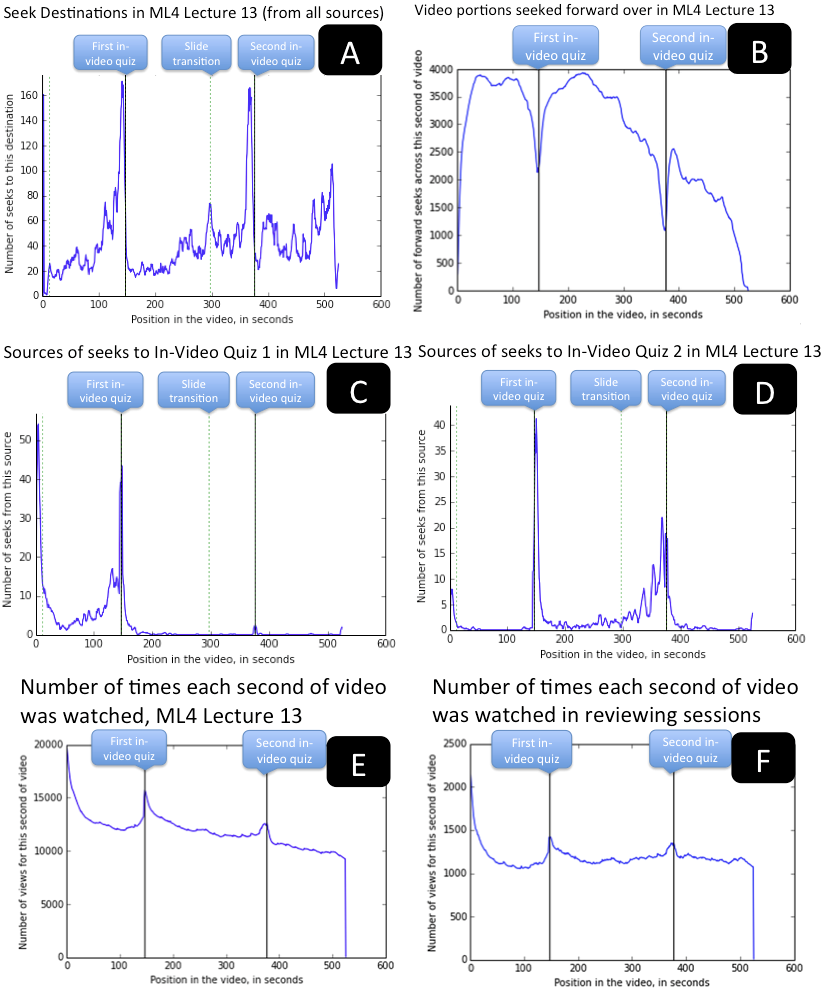
\includegraphics[width=2.0\columnwidth]{lec13-multiplot}
\caption{A) in-video quizzes are a popular destination of seeks. B) users do not tend to skip forward over in-video quizzes. C) seeks to in-video quizzes tend to be from the preceding section. D) some users are seeking directly from one in-video quiz to the next. E+F) local peaks in viewing occur around in-video quizzes.}
\label{fig:lec13-multiplot}
\end{figure*}

In order to explain why users are seeking to and from in-video quizzes, let us first visualize a representative video before moving on to videos in aggregate. This is Lecture 13 from ML4, titled ``Matrices and Vectors''. We chose it because it has 2 in-video quizzes, and neither is located at the very end of the video, so results should not be overly influenced by position of the in-video quizzes.

\autoref{fig:scatter-plot-of-seeks} presents the seek chain sources and destinations in this video as a scatter plot. It illustrates users seeking forward to in-video quizzes, going back to the preceding section to look for answers, and showing how seek chains do not tend to cross forward across in-video quizzes.

As shown in \autoref{fig:lec13-multiplot}, in-video quizzes are a popular destination of seeks. Many of these seeks originate from the from the preceding section, confirming the stats we saw in \autoref{fig:seek-sources-and-destinations-table}. This suggests that users may have found the answer to the quiz, and are seeking forward to answer the in-video quiz. However, there are also many seeks to the in-video quiz from the start of the video and the preceding in-video quiz. This suggests some users might be following a quiz-centric navigation strategy of seeking directly to the quiz to preview it before they watch the video.

% We hypothesized that if encountering in-video quizzes is causing users to try to find answers to the quiz question in the video, this should be reflected in the viewing logs. Namely, we would expect to see increased re-watching of the portion prior to the in-video quiz where the answer is located, as well as seeks that originate from the in-video quiz and go backwards to where the answer was located. This increase in rewatching of portions  of \autoref{fig:lec13-multiplot}.

\subsection{Increased rewatching near in-video quizzes}

We hypothesized that if users to try to find answers in the preceding video upon encountering an in-video quiz, this should be reflected in the viewing logs. Namely, we would expect to see increased re-watching of the portion prior to the in-video quiz where the answer is located, as well as seeks that originate from the in-video quiz and go backwards to where the answer was located. We show examples of these phenomenon in this section.

We see in \autoref{fig:lec13-multiplot} E) that the portion of the video surrounding the in-video quiz tends to receive more views. We also observe in that figure a trend of less views for portions of the video that occur later, which can be explained as in-video dropout, which occurs as a consequence of users tending to watch videos linearly \cite{juho}.

We believe the increase in number of views surrounding the in-video quiz is due to the user rewatching the portion preceding the in-video quiz, perhaps hoping to find an answer to the quiz. Indeed, if we exclude each user's first-time watch, and look only at what users are rewatching in aggregate, we still observe this peak in number of rewatches around the first in-video quiz, as shown in \autoref{fig:lec13-multiplot} F. % This effect is further amplified if we observe users' behaviors in a seperate rewatching session that occurs at least 1 hour after they initially open the. We find that in these rewatching sessions, many will just seek directly to the in-video quiz, as indicated in \autoref{fig:rewatchingsessions}.

% An alternative explanation for the increase in the number of rewatches surrounding the in-video quiz could be that in videos with a single in-video quiz (the most common format in ML4), the in-video quiz occurs towards the end of the video. The portion immediately preceding the in-video quiz also tends to be a fully-built out slide, that summarizes the content of the video. Hence, it could simply be the case that users are rewatching that particular segment, because the video content is a good summary of the entire video, rather than having anything to do with the presence of the in-video quiz. However, if we look at videos with multiple in-video quizzes, we still observe the peak of rewatching around the in-video quizzes as shown in \autoref{fig:lec13-multiplot} E, hence the rewatching is not due to just the position of the in-video quiz at the end of the video.

% We also observe a peak in the number of backwards seek chains that cross regions surrounding the in-video quiz, as shown in \autoref{fig:backseeks}. Backwards seek chains originating from the in-video quiz itself can be attributed to user behavior where the user is seeking backwards to find an answer to the in-video quiz. Backwards seek chains originating from past the in-video quiz can be attributed to users wishing to review the content tested in the in-video quiz.

Because Coursera does not enforce that users take in-video quizzes, we wondered whether users are explicitly skipping across the in-video quizzes to avoid taking them. As illustrated in \autoref{fig:lec13-multiplot} B, we found that this does not tend to be the case. On the contrary, there is actually a dip in the number of forward seeks that cross over the in-video quiz, so users are explicitly trying not to skip the in-video quizzes. This low number of forward seeks crossing over the last in-video quiz in this example might be attributed to the fact that it is at towards the end of the video, so the user may know that there is no new content to find towards the end. However, if we look at the first in-video quiz in the example, we also observe a dip in the number of forward-seeks over the in-video quiz, even though there is important content in the video after it.

% Our findings in this section suggest that users tend to attribute importance to in-video quizzes, because they rewatch the regions surrounding them, tend to backseek to review the materials preceding the quiz, and do not forward-seek over quizzes to avoid taking them.

\begin{figure}
%\centering
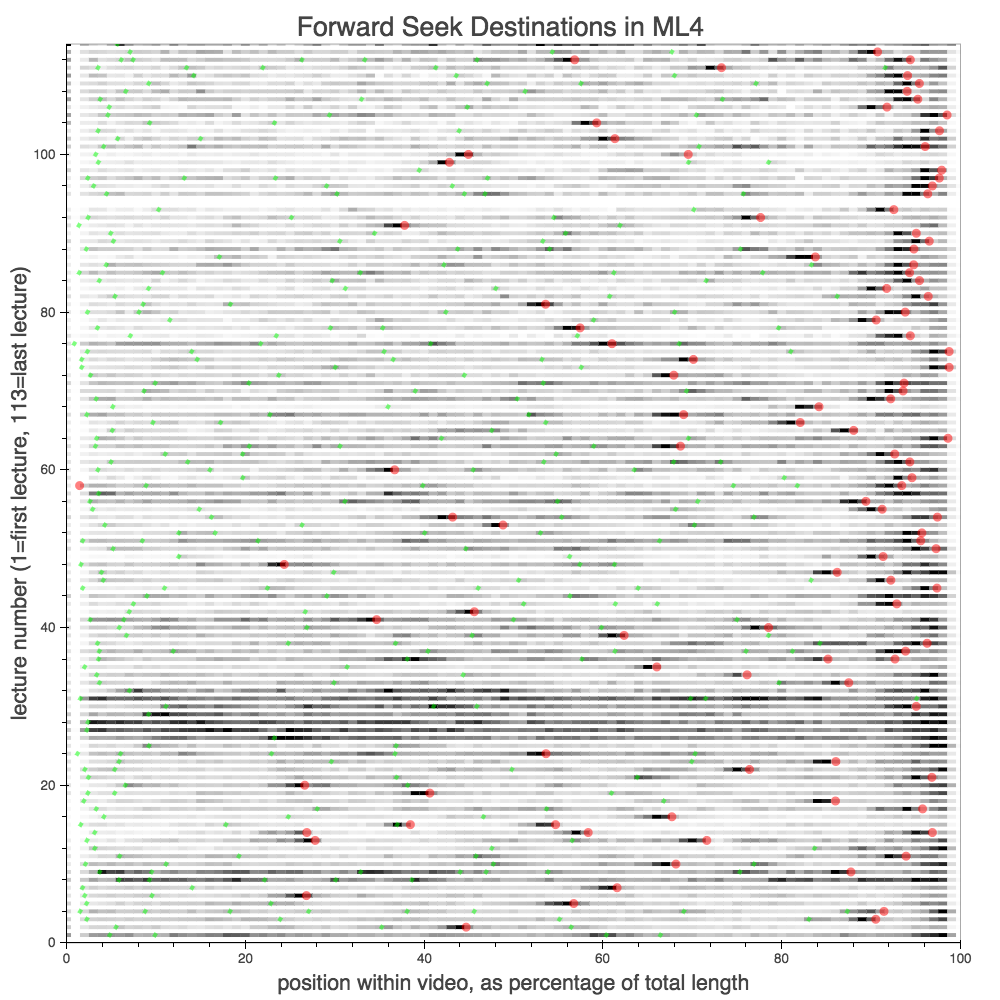
\includegraphics[width=1.0\columnwidth]{forward-seek-destinations-allvideos}
\caption{Destinations of forward seek chains in all videos. Each horizontal line represents a video; darkness of a segment indicates the number of seek chains going to that part of the video. Red dots indicate in-video quizzes, and green diamonds indicate slide transitions. Users tend to seek forward to in-video quizzes.}
\label{fig:forward-seek-destinations-allvideos}
\end{figure}

%Now, let us go beyond looking at individual videos and in-video quizzes, and visualize the seek chains across all 113 videos and 109 in-video quizzes in the course.

Now, we will look at the seek chains across all 113 videos and 109 in-video quizzes in the course.

%\pagebreak

%\section{Analysis of Seek Chains by Visualizing Seeking over All Videos}
\section{Visualizing Seeking over All Videos}

\subsection{Forward Seeking to In-Video Quizzes}

\begin{figure}
%\centering
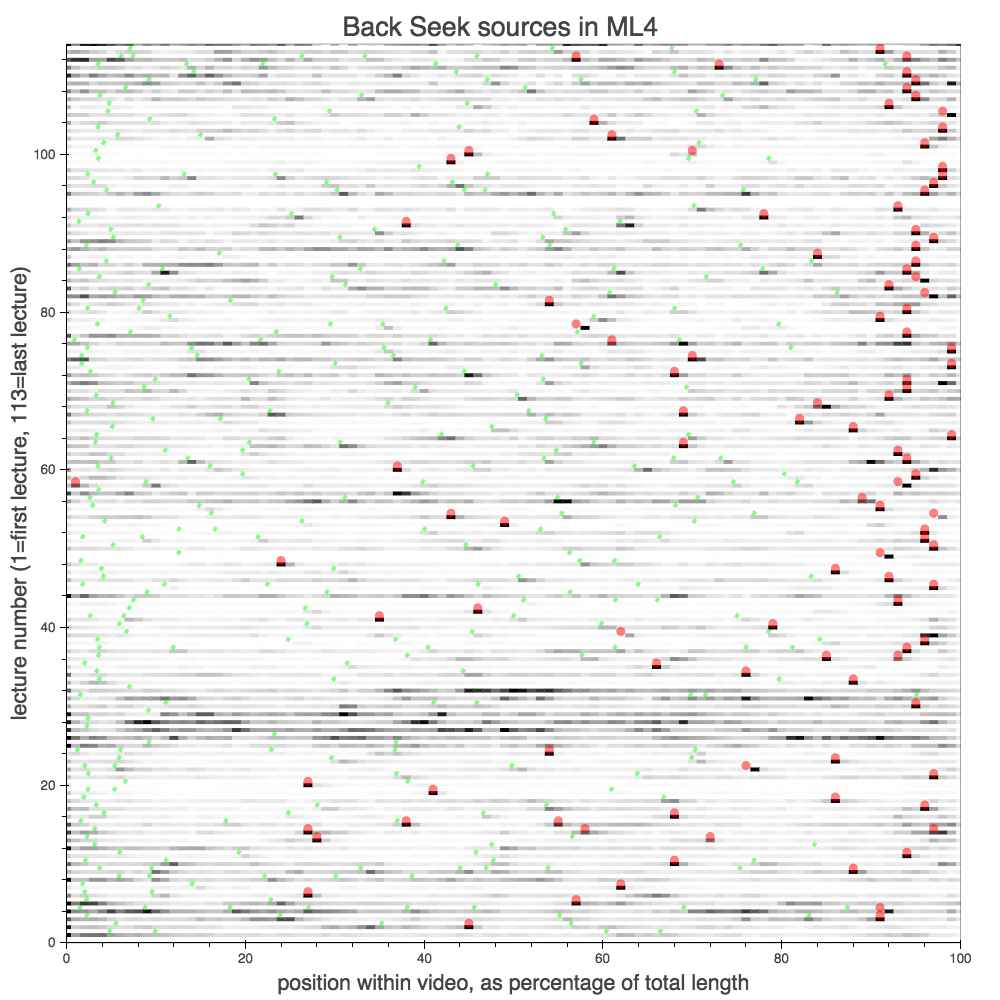
\includegraphics[width=1.0\columnwidth]{back-seek-sources-allvideos}
\caption{Sources of backward seeks. Red circles indicate in-video quizzes. In-video quizzes are a major source of backward seeks, due to users going back to the previous section to review the video.}
\label{fig:back-seek-sources-allvideos}
\end{figure}

\autoref{fig:forward-seek-destinations-allvideos} shows where users are seeking forward to in all 113 videos in the course. Each horizontal line represents a video, visualizing how many times a seek chain goes to a particular segment of the video via its darkness. We label the locations of in-video quizzes (red) and slide transitions (green). %We denote the locations of in-video quizzes (red dots) and slide transitions (green diamonds).

In-video quizzes are a popular destination of seeks, as indicated by the black streaks immediately preceding the in-video circles (recall that Coursera doesn't let users seek directly to in-video quizzes, but requires them to seek to the segment right before the quiz if they want to take it, which is why we're seeing that the seek destinations are at the preceding segment as opposed to just at the quiz itself). As we showed in \autoref{fig:seek-sources-and-destinations-table}, forward seek rates to the in-video quizzes are 4 times higher than the baseline rate.

If we look at lectures 25-30 in \autoref{fig:forward-seek-destinations-allvideos}, they don't visually match the pattern we see in the other lectures. This is because they're optional tutorial videos discussing interesting applications of Machine Learning, which don't have in-video quizzes or required material.

%\pagebreak

%\subsection{In-Video Quizzes are a Major Source of Back Seeks (Reviewing)}
\subsection{In-Video Quizzes are a Major Source of Backward Seeks}

As we can see in \autoref{fig:back-seek-sources-allvideos}, there are many seeks in the backward direction that start from the in-video quizzes (red circles). Specifically, as shown in \autoref{fig:seek-sources-and-destinations-table}, the rate of backward seek chains from in-video quizzes is 55 times higher than the baseline rate. We also see peaks in backward seeks after slide boundaries (green diamonds), which confirms prior findings of interaction peaks at slide boundaries in EdX videos which lack in-video quizzes \cite{juho}.

\subsection{Video Parts Skipped Back Over}

\begin{figure}
%\centering
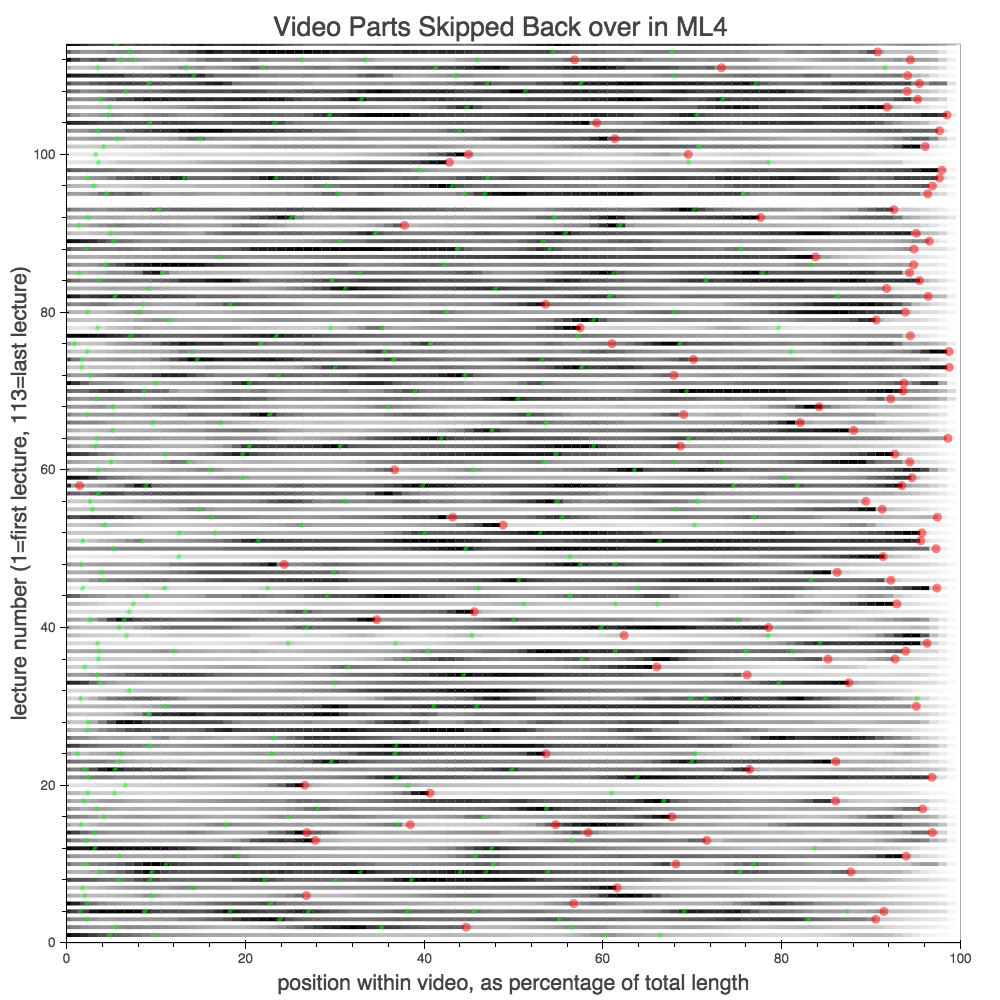
\includegraphics[width=1.0\columnwidth]{parts-skipped-back-over-allvideos}
\caption{Parts of the video skipped back over. They tend to be the portions preceding the in-video quizzes, reflecting that users are reviewing the video in response to seeing the in-video quiz}
\label{fig:parts-skipped-back-over-allvideos}
\end{figure}

As we saw in \autoref{fig:parts-skipped-back-over-allvideos} and \autoref{fig:seek-sources-and-destinations-table}, in-video quizzes are a major source of backward seek chains. As we can see in \autoref{fig:parts-skipped-back-over-allvideos}, if we look at all portions of the video that are skipped backwards over by seek chains, it is primarily the segments preceding the in-video quizzes. This can be explained by users searching in the preceding segment for the answer the in-video quiz. We suspect that the portion of the video that is seeked backwards over may reflect where the portion of the video relevant to answering the in-video quiz can be found.

Interestingly, we observe that when the last in-video quiz occurs at the midpoint of a video, as is the case with Lecture 19 in \autoref{fig:parts-skipped-back-over-allvideos}, there is little back-seeking which occurs after the video. This suggests that this phenomenon we observe of back-seeking occurring directly before a video is indeed a result of the in-video quiz causing users to backwards more, as opposed to simply being a result of the fact that the in-video quizzes tend to occur towards the end of the video.

\subsection{Seek Destinations from In-Video Quizzes}

\begin{figure}
%\centering
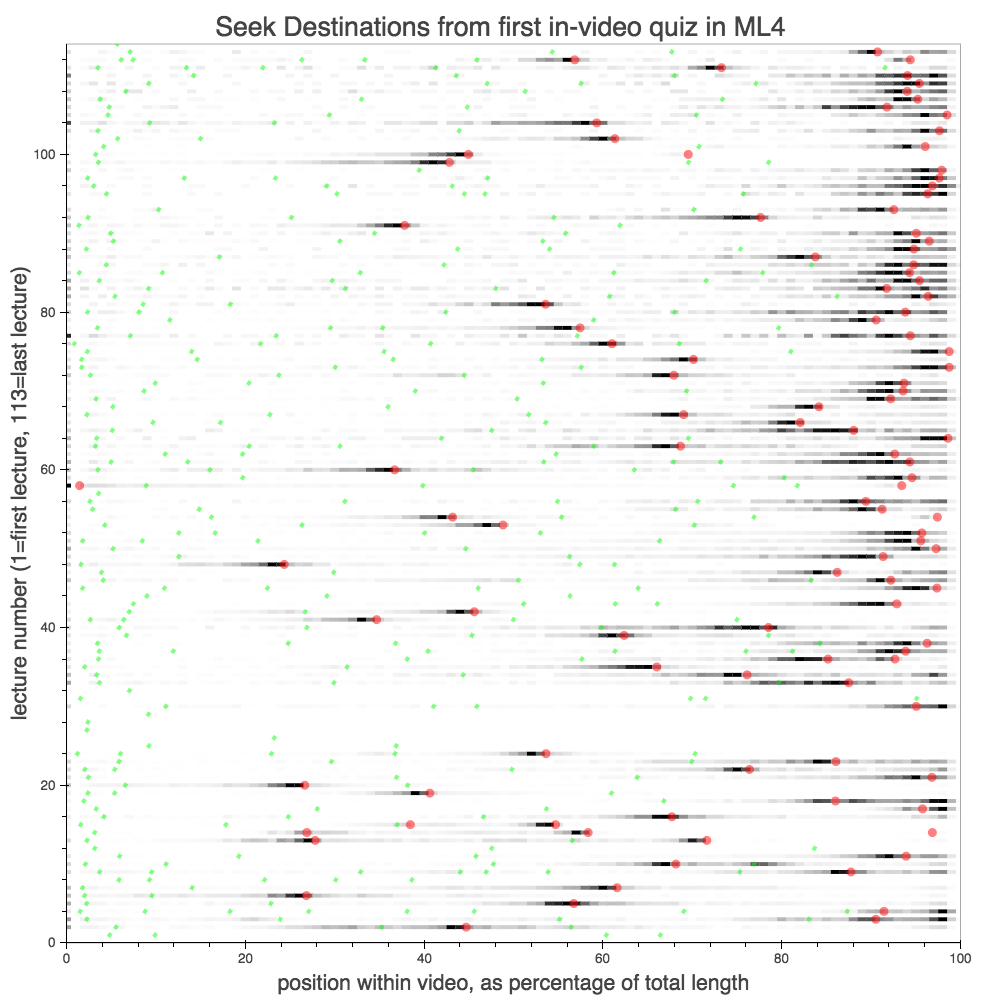
\includegraphics[width=1.0\columnwidth]{seek-destinations-from-first-quiz-allvideos}
\caption{Seek destinations from the first in-video quiz in each lecture. The portion preceding the in-video quiz is a major seek destination.}
\label{fig:seek-destinations-from-first-quiz-allvideos}
\end{figure}

As we can see in \autoref{fig:seek-destinations-from-first-quiz-allvideos}, the seek destinations from in-video quizzes are primarily backward, towards the immediately preceding portion. This is confirmed in \autoref{fig:seek-sources-and-destinations-table}, which shows that there are over 10x more seeks in the backward direction from in-video quizzes than in the forward direction. These can be explained by users who decide to go back and review the preceding segment in response to having seen the in-video quiz.

%\pagebreak

\subsection{Seek Destinations from the Start of the video}

As we can see in \autoref{fig:seek-destinations-from-start-allvideos}, many users are seeking directly from the start of the video to in-video quizzes. This means that there are some users for whom the first action they take after opening the video is to go seek to the in-video quiz. This suggests that these users might be previewing the quizzes before they watch the video, or they are using the quizzes as a navigational tool to help them decide which parts of the video they need to see and review.

\begin{figure}
%\centering
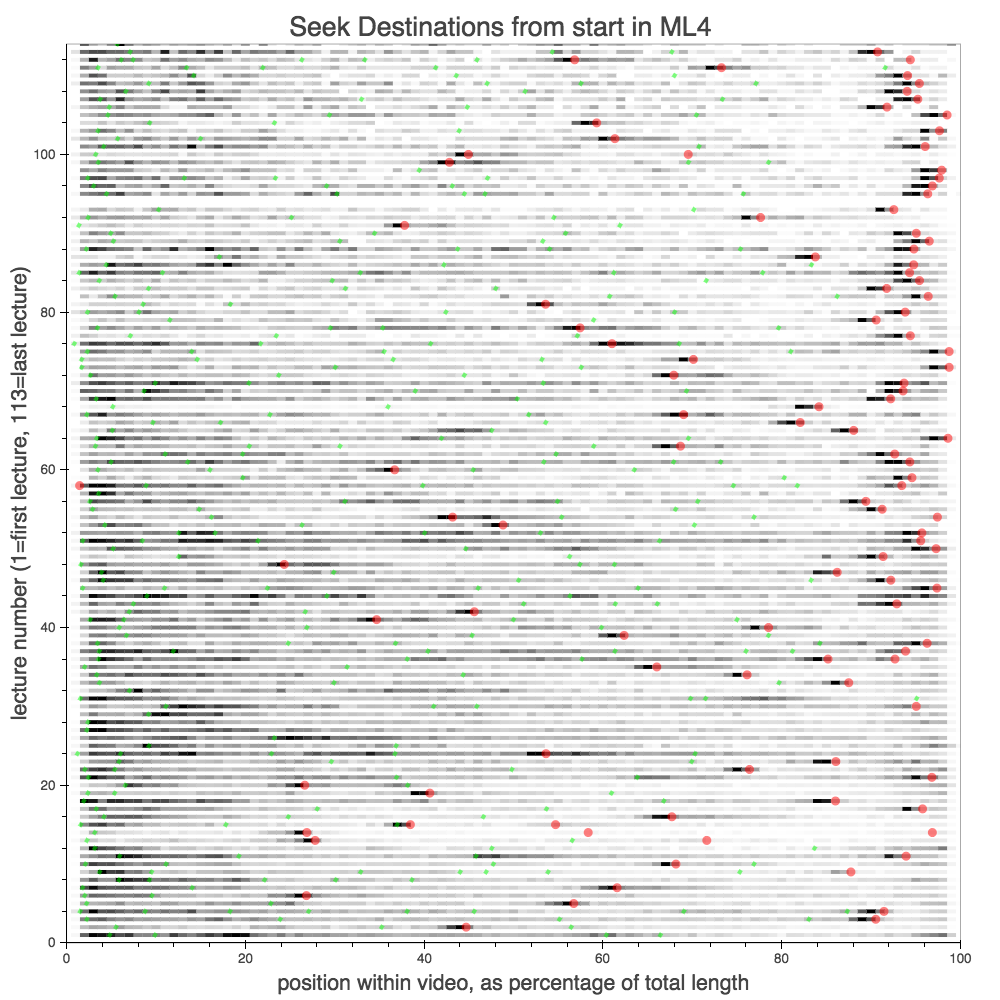
\includegraphics[width=1.0\columnwidth]{seek-destinations-from-start-allvideos}
\caption{Seek destinations from the start of the video. Many users seek directly from the start of the video to the in-video quizzes.}
\label{fig:seek-destinations-from-start-allvideos}
\end{figure}

\section{Summary of Results}

We have found that in-video quizzes are major sources and destinations of seek chains. Based on the sources and destinations of seek chains going to/from in-video quizzes, the seeking behaviors that we observe around in-video quizzes include:

\begin{itemize}
%\begin{compactitem}
\item Users seeking from one quiz to the next, presumably aiming to answer the in-video quiz questions
\item Users seeking backwards to the quiz from the immediately following section, to review its contents
\item Users seeking forward to the in-video quiz, presumably to respond to the question after having found the answer, or to remind themselves of what the quiz was asking them to find.
%\end{compactitem}
\end{itemize}

\section{Discussion}

The peaks in seeking towards in-video quizzes suggest a number of possible interface improvements that could be experimented with. Coursera currently does not allow users to easily skip directly to in-video quizzes, instead requiring them to go to the preceding few seconds of videos. As indicated by how we observed that in-video quizzes were one of the most common destinations for seek chains, particularly in the forward direction, skipping to in-video quizzes should  be made easier, perhaps via improved scrubbing techniques. % We also observed that users tend to revisit in-video quizzes during rewatching sessions. This suggests that it may be beneficial if users had an easy way to refer back to the in-video quizzes they had previously encountered while reviewing.

% A limitation in this study is that it is impossible to determine exactly what point users who simply closed their browser windows stopped watching videos at. This is due to Coursera's lack of a second-by-second heartbeat showing whether the user is still connected -- we can observe the last event from the user, but we do not know how much time elapsed between that event and the user closing their browser, so we do not know precisely where the final segment watched by the user ended. Like Coursera, EdX also does not currently implement a heartbeat for determining user disconnections either, so this is a limitation shared by other studies relying on EdX data. To better study users' interactions with videos, and to understand exactly where users lose engagement with videos and close them, these platforms need to be able to determine when users close their browsers.

Because our study did not perform any A/B tests varying the number of in-video quizzes, we do not know whether in-video quizzes have any effect on the overall video watching completion rate, or their effects on in-video dropout rates. Because few users attempt to skip in-video quizzes by forward-seeking over them as shown in \autoref{fig:seek-sources-and-destinations-table}, and that users tend to seek backwards to review when they encounter in-video quizzes, as shown in \autoref{fig:parts-skipped-back-over-allvideos}, we suspect that in-video quizzes might be beneficial for keeping users engaged with the video. % and encouraging them to watch and review the videos.

%\pagebreak

\section{Conclusion}

We have presented ways that in-video quizzes influence users' video watching behaviors, as indicated by seeking logs on various videos in the ML4 course on Coursera. We find that users' seeking and rewatching behaviors in videos are influenced by the presence of in-video quizzes. Specifically:

\begin{compactitem}
\item There are peaks in rewatching behavior in the regions surrounding the in-video quiz. In particular, we see a large amount of back-seeking from in-video quizzes to the immediately preceding video section. This is likely due to users seeking answers to in-video quizzes.
% \item Many users skip directly to the in-video quizzes during rewatching sessions. Hence, they may be using these as a way to test themselves, to determine whether or not they need to review that video. 
\item Users do not tend to seek forwards over in-video quizzes to skip over them.
\item In-video quizzes are a common source of seek chains within videos. Users tend to seek backward to find answers, or forward to the next in-video quiz.
\item In-video quizzes are a common destination of seek chains within videos. Users tend to seek from the preceding video segment where the answer can be found, from the beginning of the video, or from the preceding in-video quiz.
\end{compactitem}

%\pagebreak

%\section{Acknowledgements}

%Anonymized for submission

\balance{}

%\bibliographystyle{acm-sigchi}
\bibliographystyle{SIGCHI-Reference-Format}
\bibliography{invideo}

\end{document}
